\documentclass[14pt]{extarticle}
\usepackage[utf8]{inputenc}
\usepackage{amsmath}
\usepackage{amsfonts}
\usepackage{graphicx}
\usepackage{setspace}
\usepackage{geometry}
\usepackage{enumitem}
\usepackage{amssymb}
\usepackage{xcolor}
\usepackage{mathtools}
\usepackage{float}
\usepackage{listings}
\usepackage{tabularx}
\usepackage{bm}

\geometry{
    top=1in,
    bottom=1in,
    left=1in,
    right=1in,
    headheight=14pt,
    headsep=25pt,
    footskip=30pt
}

\title{Bayes Theorem}
\author{Yana Jin}
\date{Tuesday, 15th October 2024}

\onehalfspacing

\newcommand{\coverpage}{%
    \begin{titlepage}
        \centering
        
\includegraphics[width=1\textwidth]{cover.png}
    \end{titlepage}
}

\begin{document}

\coverpage

\section*{Testing and Analysis of Variance}

\noindent
So far, we have seen testing of a single parameter \textcolor{red}{$(\beta_j)$} or a contrast.
This boils down to:\\
$H_0: \theta = \theta_0 \quad (\theta \equiv \text{parameter of interest})$\\
$H_1: \theta \neq \theta_0$\\
We have used the \textit{t-statistic}:
\[
t = \frac{\hat{\theta} - \theta_0}{SE(\hat{\theta})} \overset{H_0}{\sim} t_{\text{df}}\quad \textcolor{red}{\text{df depends on } \hat{\sigma}^2}
\]
Here we drill down more into comparing the fit of mean functions rather than comparing parameter estimates.

\subsection*{F-tests \textcolor{red}{(also called ANOVA or LR Tests)}}

\textbf{Set up:}  
Suppose we have: $Y \text{ and } X'_{p+1} = \left( X'_1, X'_2 \right)$\\
where: \textcolor{red}{$X'_1$ is (p!q) regressors, $X'_2$ is q regressors}\\
\textbf{Consider Testing}
\[
H_0: E(Y \mid X_1 = x_1, X_2 = x_2) = x'_1 \beta_1
\]
\[
H_1: E(Y \mid X_1 = x_1, X_2 = x_2) = x'_1 \beta_1 + x'_2 \beta_2
\]
Different since $H_0$ and $H_1$ refer to mean function specifications, \textcolor{red}{[not restrictions on the parameters]}\\
\textcolor{blue}{Also require $H_0$ to be a part of $H_1$, [ie. $H_0$ is obtained by setting $\beta_2 = 0$]}\\
\textbf{Idea:}\\
 - Recall that \textbf{RSS} (Residual Sum of Squares) measures the amount of variation in the response not explained by the regressors.\\
$\Rightarrow \text{If } H_0 \text{ is false, then } RSS_{H_1} < RSS_{H_0}$\\
$\Rightarrow$ Test Statistic
\[
F = \frac{\frac{RSS_{H_0} - RSS_{H_1}}{df_{H_0} - df_{H_1}}}{\frac{RSS_{H_1}}{df_{H_1}}}
 = \frac{\frac{SSReg}{df_{\text{reg}}}}{\hat{\sigma}^2}
\]
\textcolor{red}{$F$: due to R.A. Fisher . $\frac{SSReg}{df_{\text{reg}}}\text{also called mean square for regression}$}\\

\noindent
\textbf{Note:}\\
$SSReg = RSS_{H_0} - RSS_{H_1}$\\
$\hat{\sigma}^2 = \frac{RSS_{H_1}}{df_{H_1}}$ [under $H_1$] \textcolor{red}{$\hat{\sigma}^2$ : \text{other choices available}}\\
If assume $e|X \sim N(0, \sigma^2 I)$, then \textcolor{blue}{under $H_0$}, 
\[
F \overset{H_0}{\sim} F(df_{\text{reg}}, df_{H_1})
\]
Large \textcolor{red}{observed} values of $(F_{\text{obs}})$ indicate evidence against $H_0$.

\subsection*{Special Cases}
Overall Test, Simple Regression
\[
H_0: E(Y \mid X = x) = \beta_0 \quad \textcolor{red}{\text{(called "null" model)}}
\]
\[
H_1: E(Y \mid X = x) = \beta_0 + \beta_1 x
\]
\[
\textcolor{red}{\text{(observed value) }}
RSS_{H_0} = \sum_{i=1}^{n} (y_i - \hat{\beta}_0)^2  = \sum_{i=1}^{n} (y_i - \bar{y})^2 = SYY
, df_{H_0} = n - 1
\]
\[
\textcolor{red}{\text{(observed value) }} RSS_{H_1} = RSS \quad \text{(from SLR)}, 
df_{H_1} = n - 2
\]
\[
F = \frac{(SYY - RSS) / \left[(n - 1) - (n - 2)\right]}{\hat{\sigma}^2}
\]
\[
= \frac{SSReg}{\hat{\sigma}^2} = \frac{SYY - RSS}{\hat{\sigma}^2}
\]
Under $H_0$, $F \sim F(1, n - 2)$\\
If $F_{\text{obs}}$ is large with respect to the null sampling distribution, this provides evidence against $H_0$.

\subsection*{Example: Forbes Data}

Scottish physicist \textbf{James Forbes} ran experiments examining the relationship between atmospheric pressure and the boiling point of water.
\begin{figure}[H]
    \centering
    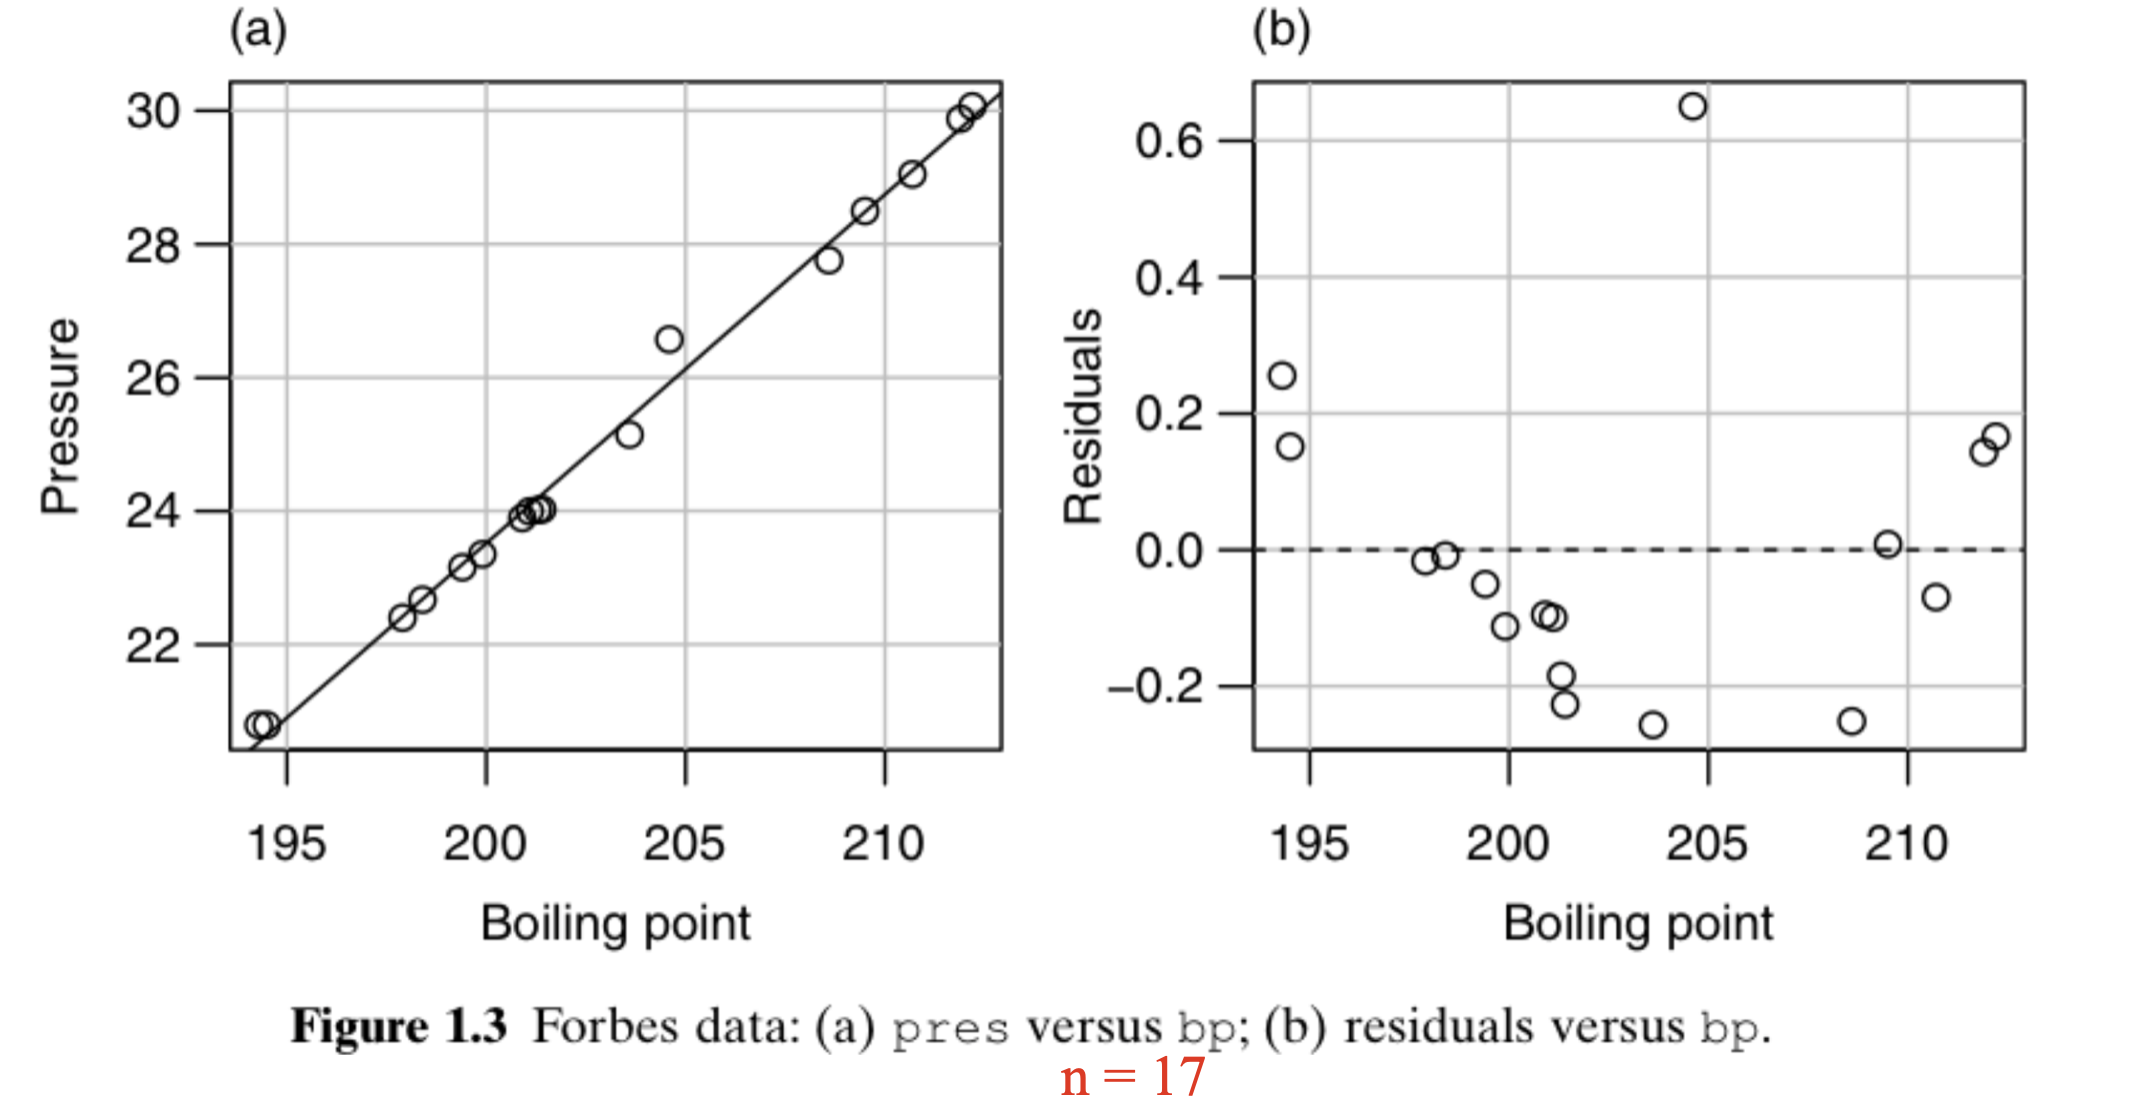
\includegraphics[width=0.95\textwidth]{fig1.png}
\end{figure}
\[
SYY = 427.794, RSS = 2.155, \hat{\sigma}^2 = 0.144
\]
\[
\Rightarrow F_{\text{obs}} = \frac{427.794 - 2.155}{0.144}
= 2962.79
\]
\[
F \overset{H_0}{\sim} F(1, 15)
\Rightarrow p < 0.0001\text{ (very strong evidence against } H_0)
\]

\subsection*{Overall Test, Simple Regression}

\noindent
$H_0: E(Y \mid X = x) = \beta_0$\\
$H_1: E(Y \mid X = x) = \beta_0 + \beta_1 x \textcolor{red}{\text{(where } x \text{ is a vector of length } p)}$\\
Fit Under $H_0 \quad \Rightarrow \hat{\beta}_0 = \bar{y} \quad \Rightarrow RSS_{H_0} = SYY , \quad df_{H_0} = n - 1$\\
Under $H_1$, $RSS_{H_1}$ and $df_{H_1}$ are from the full model fit.

\subsection*{Fuel consumption data example}
$F_{\text{obs}} = 11.99, F \overset{H_0}{\sim} F(4, 46) \Rightarrow p < 0.0001 \therefore \text{strong evidence against } H_0$. 

\subsection*{Example: UN data}
\begin{figure}[H]
    \centering
    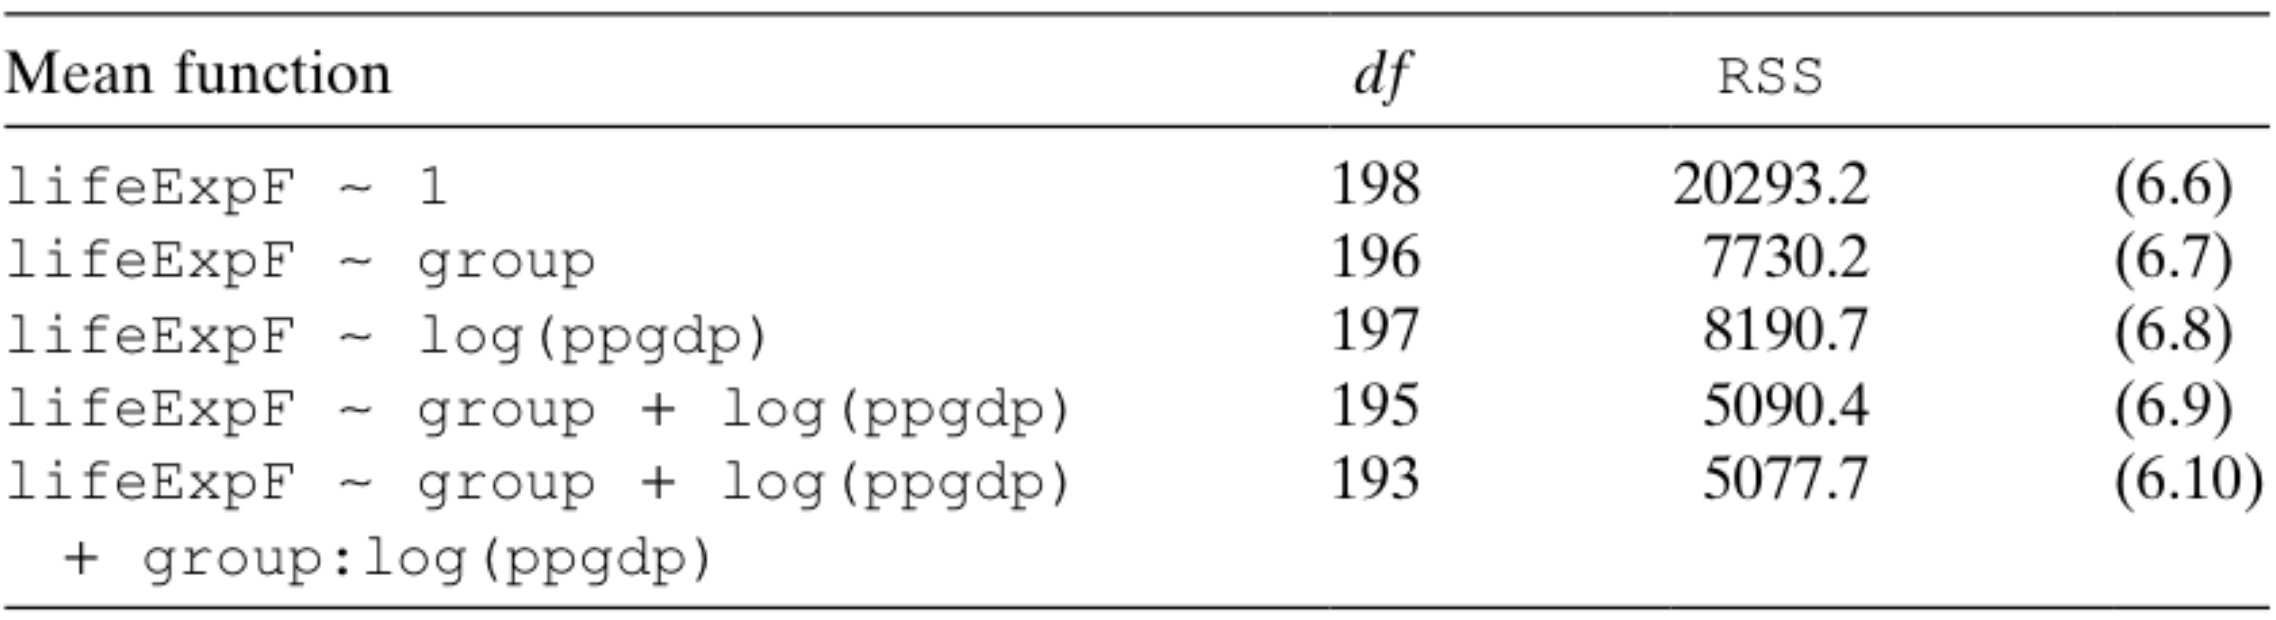
\includegraphics[width=1\textwidth]{fig2.png}
\end{figure}
\noindent
Mean function (6.6) is the null model, so: $RSS_{\text{null}} = SYY, df_{\text{null}} = n - 1$\\
Mean function (6.7) has a separate mean for each level of \textcolor{blue}{group}.\\
Mean function (6.8) has a common slope and intercept for each level of \textcolor{blue}{\text{group}}.\\
Mean function (6.9) has a separate intercept but a common slope.\\
Mean function (6.10) has separate slopes and intercepts.\\
\textbf{Different comparisons can be made.}\\
\textbf{Example1}\\
$H_0: \text{mean function (6.9)}$ \\
$H_1: \text{mean function (6.10)}$
\[
F_{\text{obs}} = \frac{(5090.4 - 5077.7) / (195 - 193)}{5077.7 / 193}
 = 0.24
\]
\[
F \overset{H_0}{\sim} F(2, 193) 
\Rightarrow p = 0.79 \text{ , no evidence against } H_0
\]
\textbf{Example2}\\
$H_0: \text{Mean function (6.8)}$\\
$H_1: \text{Mean function (6.9)}$
\[
F_{\text{obs}} = \frac{(8190.7 - 5090.4) / (197 - 195)}{5090.4 / 195} = 59.38
\]
\[
F \overset{H_0}{\sim} F(2, 195)
\Rightarrow p < 0.0001 \therefore \text{strong evidence against } H_0
\]
\textbf{Note:}\\
Two tests just illustrated use different denominators for F-tests.\\
However, when testing summarized in ANOVA table, the largest model (6.10) would be used for all tests.\\
When doing that for the second test: $F_{\text{obs}} = 58.92 \quad \text{(little change)}$

\section*{General Likelihood Ratio Tests}

\textbf{Fact:} F-tests described are the same as Likelihood Ratio Tests for linear models with normal errors.

\subsection*{The Analysis of Variance}

Suppose we fit the following model:
\[
Y \sim A + B + C + A:B + A:C + B:C + A:B:C,
\]
where each of $A$, $B$, or $C$ could represent a continuous predictor with a single degree of freedom, or a factor, polynomial, or spline basis with more than one degree of freedom. An interaction like $A:B$ can have many degrees of freedom.

The approach to testing we adopt follows from the \textit{marginality principle}. A lower-order term, such as the $A$ main effect, is never tested in models that include any of its higher-order relatives like $A:B$, $A:C$, or $A:B:C$. All regressors that are not higher-order relatives of the regressor of interest, such as $B$, $C$, and $B:C$, are always included in both $H_0$ and $H_1$.

Based on the marginality principle, testing should begin with the highest-order interaction first:
\[
H_0: Y \sim A + B + C + A:B + A:C + B:C,
\]
\[
H_1: Y \sim A + B + C + A:B + A:C + B:C + A:B:C.
\]

If the $A:B:C$ interaction is judged to be nonzero, no further testing is required, since $A:B:C$ is a higher-order relative of all remaining regressors in the mean function.

If the $A:B:C$ interaction is judged nonsignificant, then proceed to examine the two-factor interactions, such as:
\[
H_0: Y \sim A + B + C + A:C + B:C,
\]
\[
H_1: Y \sim A + B + C + A:B + A:C + B:C,
\]
which tests the interaction $A:B$.

Tests for a main effect like $A$ would be carried out only if all its higher-order relatives, $A:B:C$, $A:B$, and $A:C$, are judged to be unimportant. One would then test:
\[
H_0: Y \sim B + C + B:C,
\]
\[
H_1: Y \sim A + B + C + B:C.
\]
where $B:C$ is included in both the $H_0$ and the $H_1$.  
Table shows the analysis of variance for the UN data.
\begin{figure}[H]
    \centering
    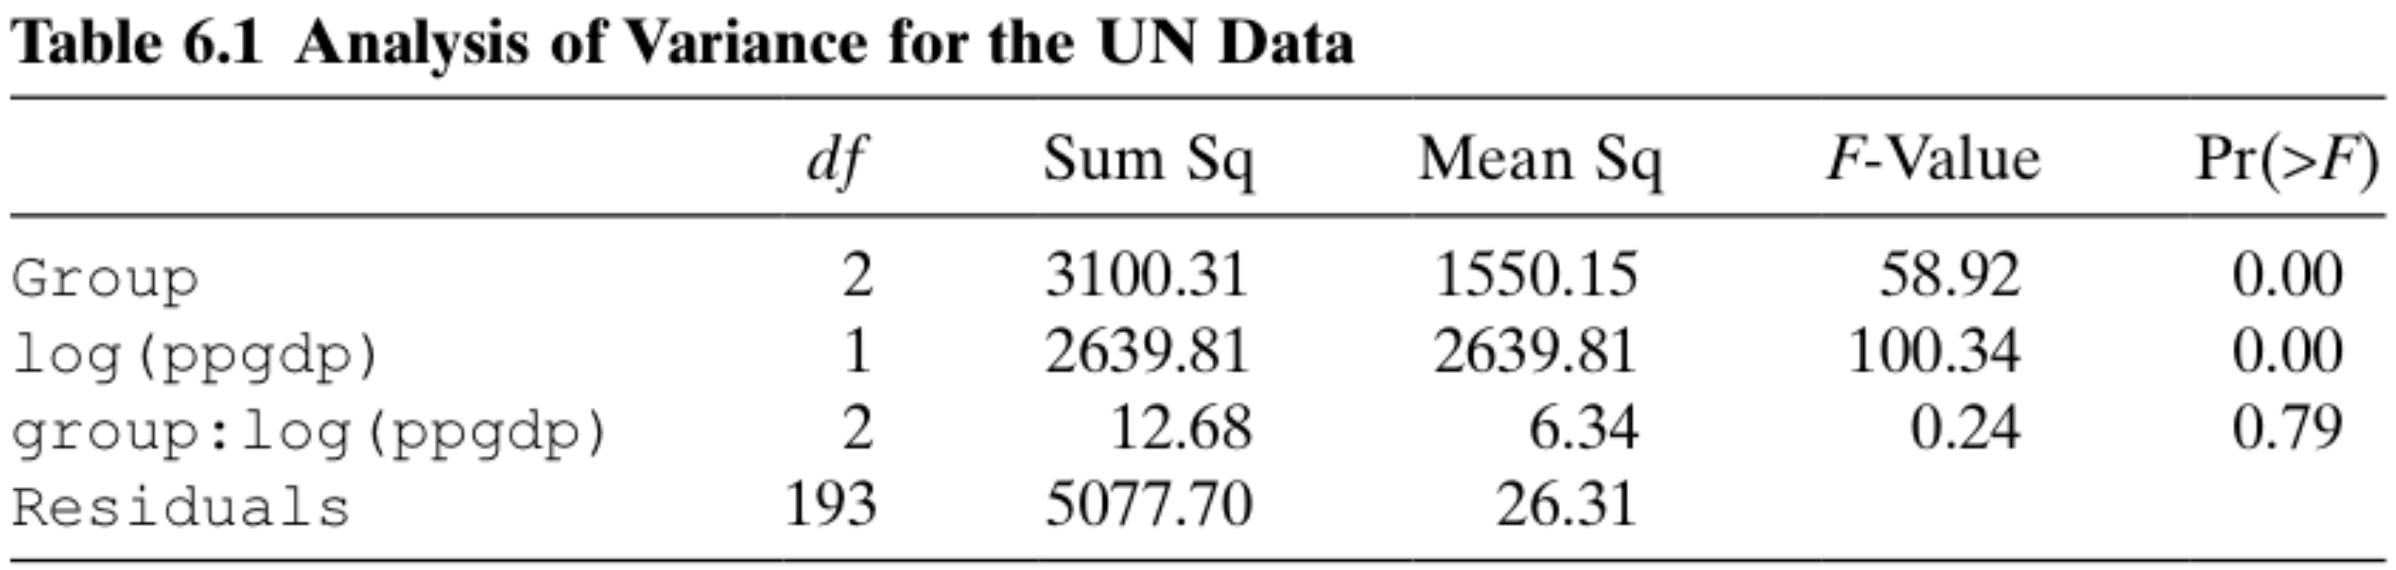
\includegraphics[width=1\textwidth]{fig3.png}
\end{figure}
An analysis of variable table derived under the marginality principle has the unfortunate name of Type II analysis of variance. At least two other types of ANOVA are commonly available in software packages:

\textit{Type I ANOVA}, also called sequential ANOVA, fits the model according to the order that the regressors are entered into the mean function. For example, if we fit the model:

$Y \sim A + B + C + A:B + A:C + B:C + A:B:C$,

then the sequence of models that would be represented in the ANOVA table would have regressors: 
$\{A\}, \{A, B\}, \{A, B, C\}, \{A, B, C, A:B\}, \{A, B, C, A:B, A:C\}, \{A, B, C, A:B, A:C, B:C\}$ and $\{A, B, C, A:B, A:C, B:C, A:B:C\}$.

If the terms were written in a different order, then the analysis would have different conditioning. Type I ANOVA generally has only pedagogical interest and should not be used.

Type III ANOVA violates the marginality principle. It computes the test for every regressor adjusted for every other regressor. For example, the test for the $A$ main effect would include the interactions $A:B$, $A:C$, and $A:B:C$ in both $H_0$ and $H_1$. There is a justification for this testing paradigm, called the marginal means method, but some of these tests depend on the parameterization used for the regressors and so they are not recommended for general use.

The wool data is from a designed experiment in which all the factors are orthogonal to each other. Table shows the ANOVA table for the full second-order model. Because the regressors are orthogonal, Type I, Type II, and Type III tests are identical.
\begin{figure}[H]
    \centering
    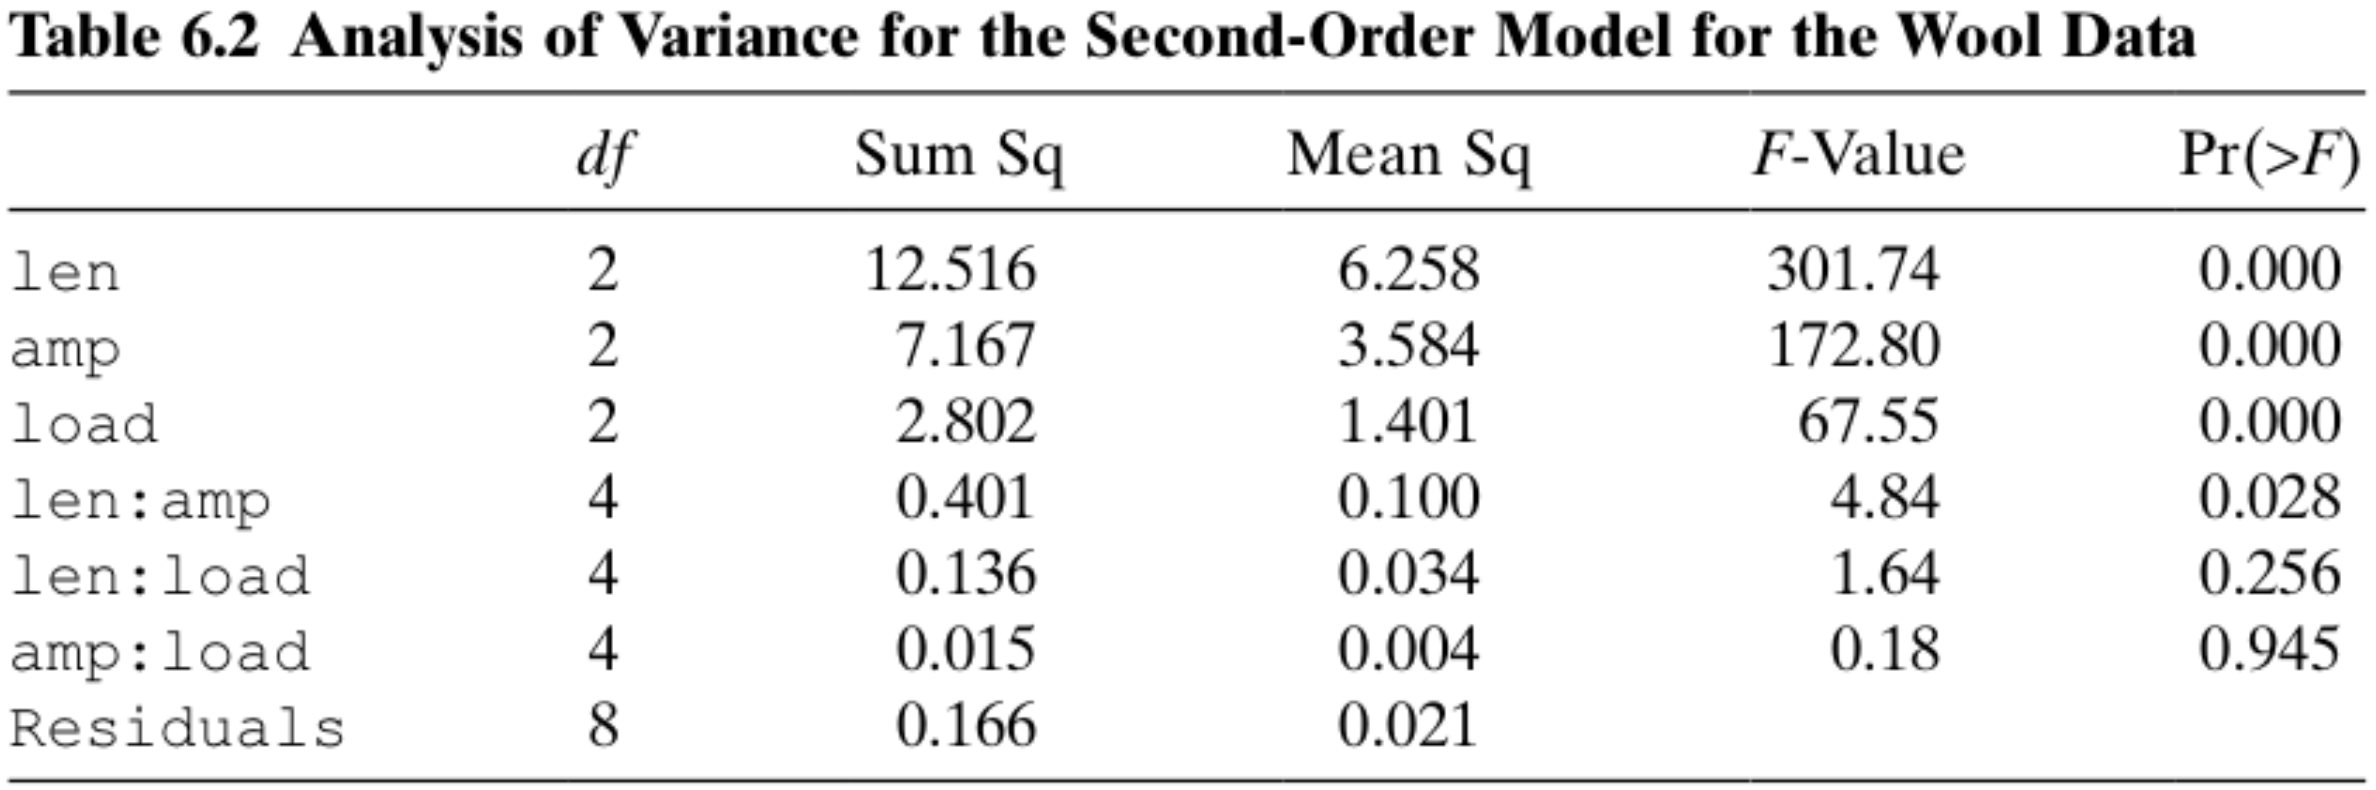
\includegraphics[width=1\textwidth]{fig4.png}
\end{figure}
\begin{figure}[H]
    \centering
    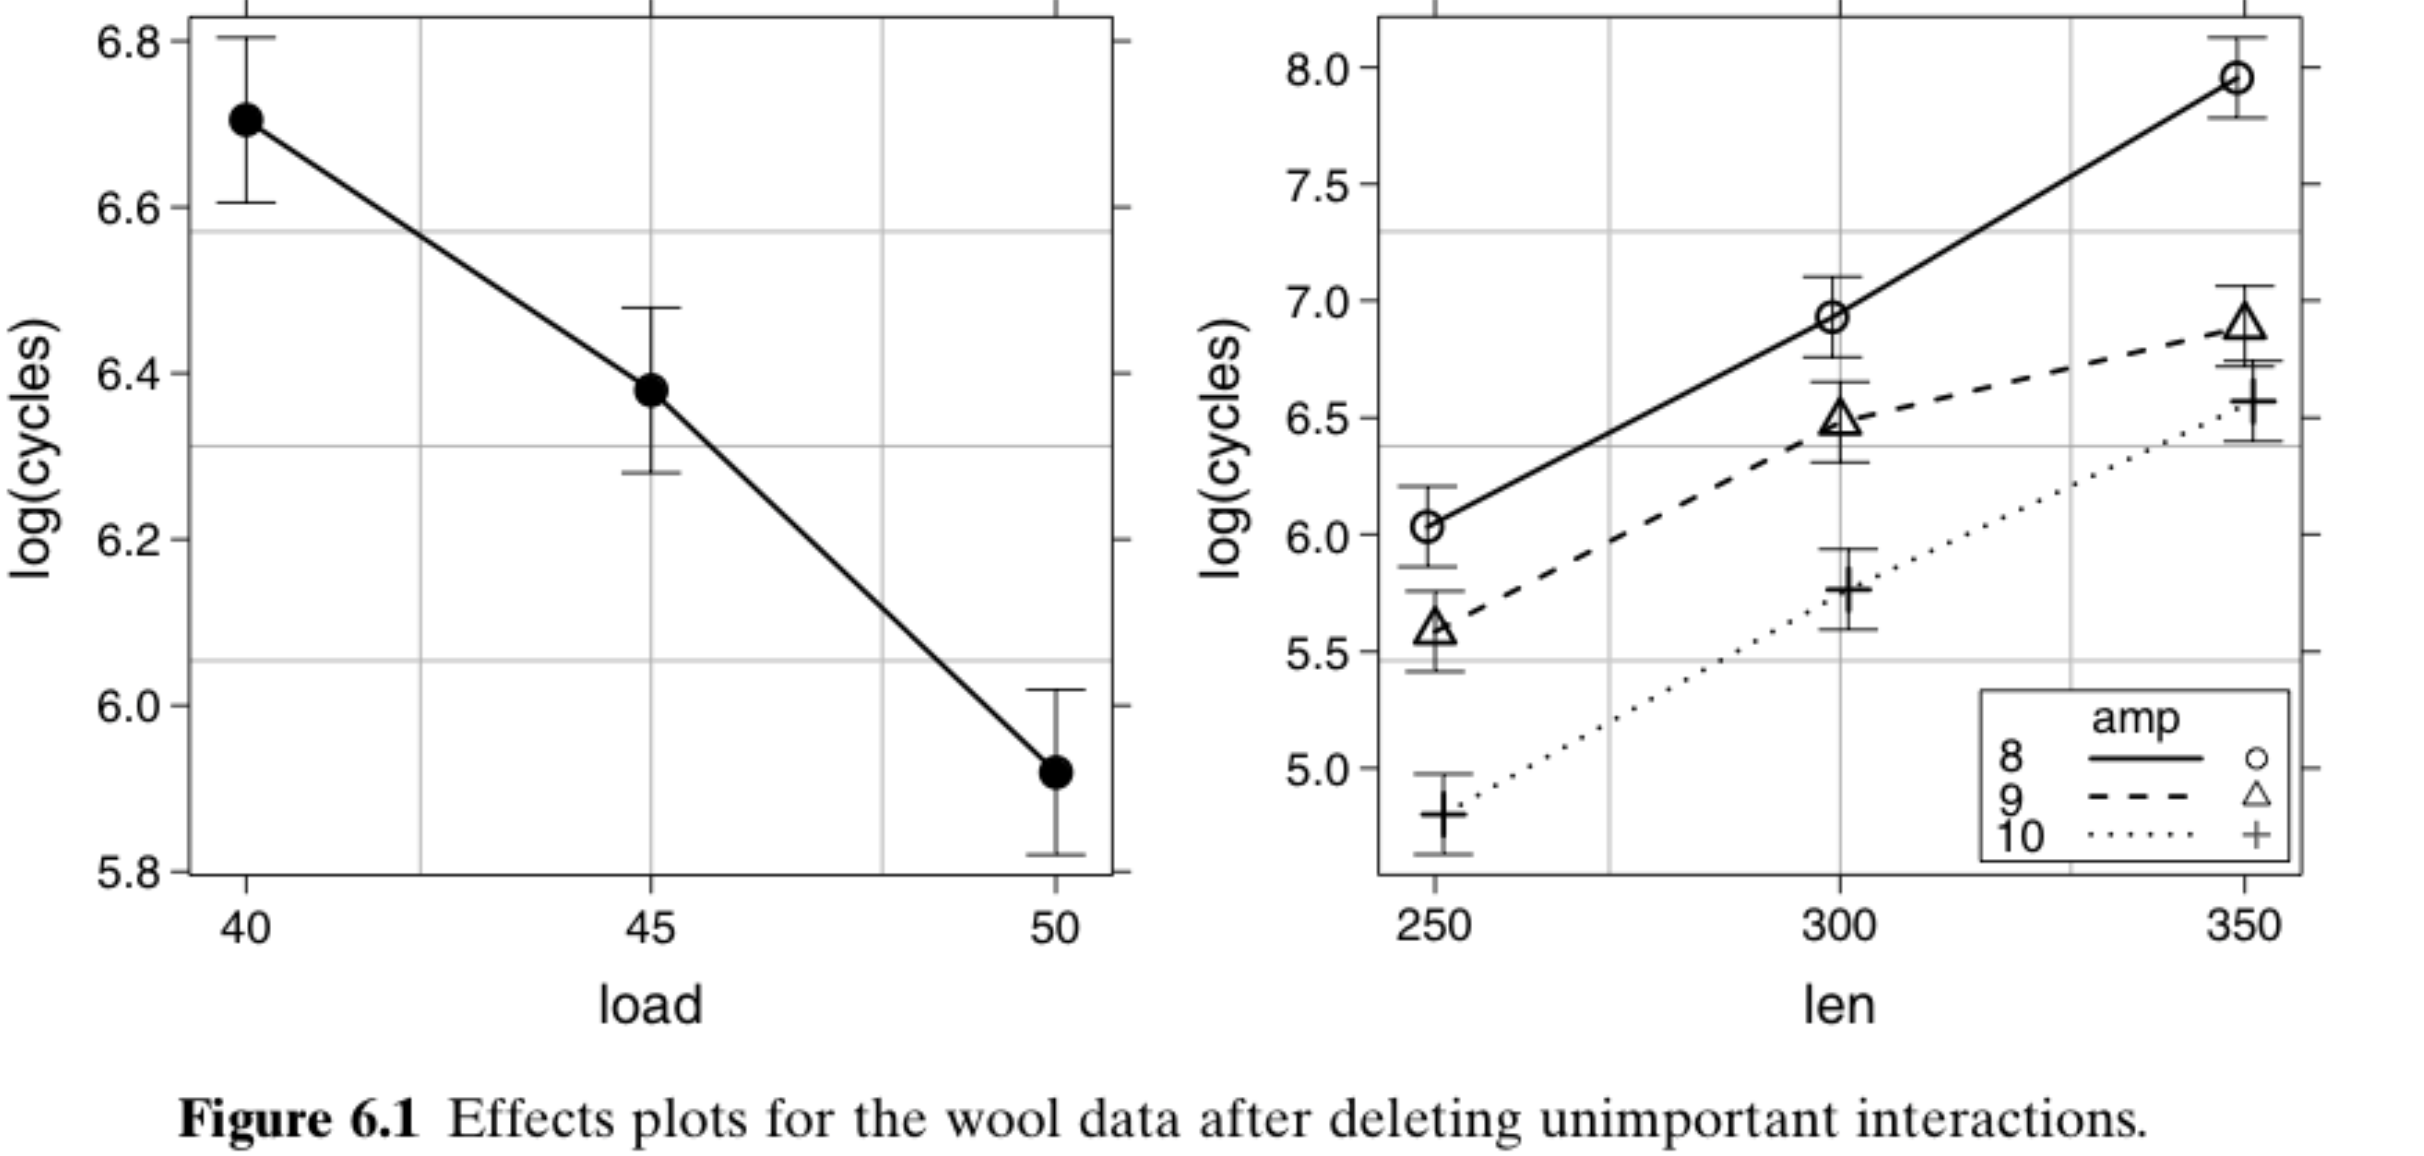
\includegraphics[width=1\textwidth]{fig5.png}
\end{figure}

\subsection*{Power and Non-Null Distributions}

\noindent
For the full-reduced model test, the test statistic is 
\[
F = \frac{(RSS_{H_0} - RSS_{H_1}) / (df_{H_0} - df_{H_1})}{RSS_{H_1} / df_{H_1}}
\]
For a fixed significance level, the probability of rejecting a false $H_0$ is called the power of the test:
\[
power = \text{Prob}(\text{detect a false } H_0)
= \text{Prob}(F > f^* \mid H_1 \text{ is true}),
\]

where $f^*$ denotes the critical value of the test.
\vspace{0.5cm}

When $H_1$ is true, the numerator and denominator of the test statistic remain independent. The denominator estimates $\sigma^2$ under both the $H_0$ and the $H_1$. The distribution of the numerator sum of squares is different under the $H_0$ and the $H_1$. Apart from \textit{df}, the numerator under the $H_1$ is distributed as $\sigma^2$ times a noncentral $\chi^2$.

The expected value of the numerator will be
\[
\sigma^2(1 + \lambda),
\]

where $\lambda$ is called the noncentrality parameter and can be expressed as
\[
\lambda = \frac{\beta_2' X_2' \left( I - X_1 \left( X_1' X_1 \right)^{-1} X_1' \right) X_2 \beta_2}{q \sigma^2}.
\]

In the case that $X_2$ consists of a single variable, i.e., $q = 1$, $\beta_2$ is a scalar, and
\[
\lambda = (n - 1) \left( \frac{\beta_2}{\sigma} \right)^2 SD_2^2 \left( 1 - R_{x_2, x_1}^2 \right),
\]
where $SD_2$ is the standard deviation of $X_2$, and $R_{x_2, x_1}^2$ is the value of $R^2$ for the OLS regression with response $X_2$ and regressor $X_1$.

Power increases with $\lambda$, so it increases with sample size $n$, the size of the parameter relative to the error standard deviation $\left(\frac{\beta_2}{\sigma}\right)^2$, and $SD_2^2$. 

In most designed experiments, interesting tests concern effects that are orthogonal. Then
\[
\lambda = (n - 1) \frac{\beta_2' S_2 \beta_2}{q \sigma^2},
\]
where $S_2$ is the sample covariance matrix for $X_2$.

\section*{Wald Tests}
Wald tests about regression coefficients are based on the distribution of the estimate $\hat{\beta}$. In most regression problems, the estimator is at least approximately normally distributed,
\[
\hat{\beta} \sim N(\beta, V).
\]
\vspace{1cm}

Generally, $V$ is unknown, but an estimate $\hat{V}$ is available. For OLS estimators, we have
\[
\hat{V} = \hat{\sigma}^2 (X' X)^{-1}.
\]

\subsection*{One Coefficient}
To test a hypothesis, say $H_0: \beta_j = \beta_{j_0}$ versus $H_1: \beta_j \neq \beta_{j_0}$, compute

\[
t = \frac{\hat{\beta}_j - \beta_{j_0}}{\sqrt{\hat{v}_{jj}}},
\]

where $\hat{v}_{jj}$ is the $(j,j)$th element of $\hat{V}$. This test is compared with the $t$-distribution with degrees of freedom equal to the degrees of freedom in estimating $\sigma^2$ to get $p$-values.

In problems like logistic regression, where there is no $\sigma^2$ to estimate, the Wald test is compared with the standard normal distribution.

\subsection*{One Linear Combination}

Suppose $\bm{a}$ is a vector. Then the linear combination $l = \bm{a}'\bm{\beta}$ has the estimate $\hat{l} = \bm{a}'\hat{\bm{\beta}}$ and

\[
\hat{l} \sim N(l, \bm{a}'V\bm{a}).
\]

Therefore, for $H_0: l = l_0$, the statistic is

\[
t = \frac{\hat{l} - l_0}{\sqrt{\bm{a}'\hat{V}\bm{a}}},
\]

which is compared with the $t$-distribution with degrees of freedom given by the degrees of freedom for $\hat{\sigma}^2$.

\subsection*{General Linear Hypothesis}

Suppose we wish to test \(H_0: L\boldsymbol{\beta} = \boldsymbol{c}\) versus \(H_1: L\boldsymbol{\beta} \neq \boldsymbol{c}\), where \(L\) is a \(q \times p'\) matrix of constants. 

The test statistic is 

\[
F = \frac{(L\hat{\boldsymbol{\beta}} - \boldsymbol{c})' (L \hat{V} L')^{-1} (L\hat{\boldsymbol{\beta}} - \boldsymbol{c})}{q}.
\]

Under \(H_0\) and normality, this statistic can be compared with an \(F(q, n - p')\) distribution to get significance levels.

\subsection*{Equivalence of Wald and Likelihood-Ratio Tests}

For linear regression, the Wald tests and the likelihood ratio tests give the same answer for any fixed hypothesis test. This equality does not carry over to other regression settings like logistic regression. 
Wald and likelihood ratio tests for logistic regression are equivalent, in the sense that for large enough samples they will give the same inference, but not equal, as the computed statistics generally have different values. Likelihood ratio tests are generally preferable.

\section*{Interpreting Tests}

\subsection*{Interpreting \textit{p}-values}

Under the appropriate assumptions, the \textit{p}-value is the conditional probability of observing a value of the computed statistic as extreme or more extreme than the observed value, given that the $H_0$ is true. 
A small \textit{p}-value provides evidence against the $H_0$.

In many research areas it has become traditional to adopt a fixed significance level when examining $p$-values. The most common choice for the significance level is $\alpha = 0.05$, which would mean that, were the $H_0$ to be true, we would incorrectly find evidence against it about 5\% of the time, or about one test in 20.

There is an important distinction between statistical significance, the observation of a sufficiently small $p$-value, and scientific significance, observing an effect of sufficient magnitude to be meaningful. Judgment of the latter usually will require examination of more than just the $p$-value.

\subsection*{Why Most Published Research Findings Are False}

\noindent
\textbf{Following Ioannidis (2005):}\\
Set up:\\
 - Multiple tests all at level $\alpha$\\
 - All with the same power to reject $H_0$ (say $\gamma$)\\
1. Suppose fraction $f$ are potential discoveries.\\
2. True discovery happens with probability $f\gamma$.\\
3. False discovery happens with probability $(1 - f) \alpha$.\\
4. $P(\text{discovery}) = f\gamma + (1 - f) \alpha$\\
\[
\therefore P(\text{true discovery} \mid \text{discovery}) =
\frac{f\gamma}{f\gamma + (1 - f) \alpha}
\]
\begin{figure}[H]
    \centering
    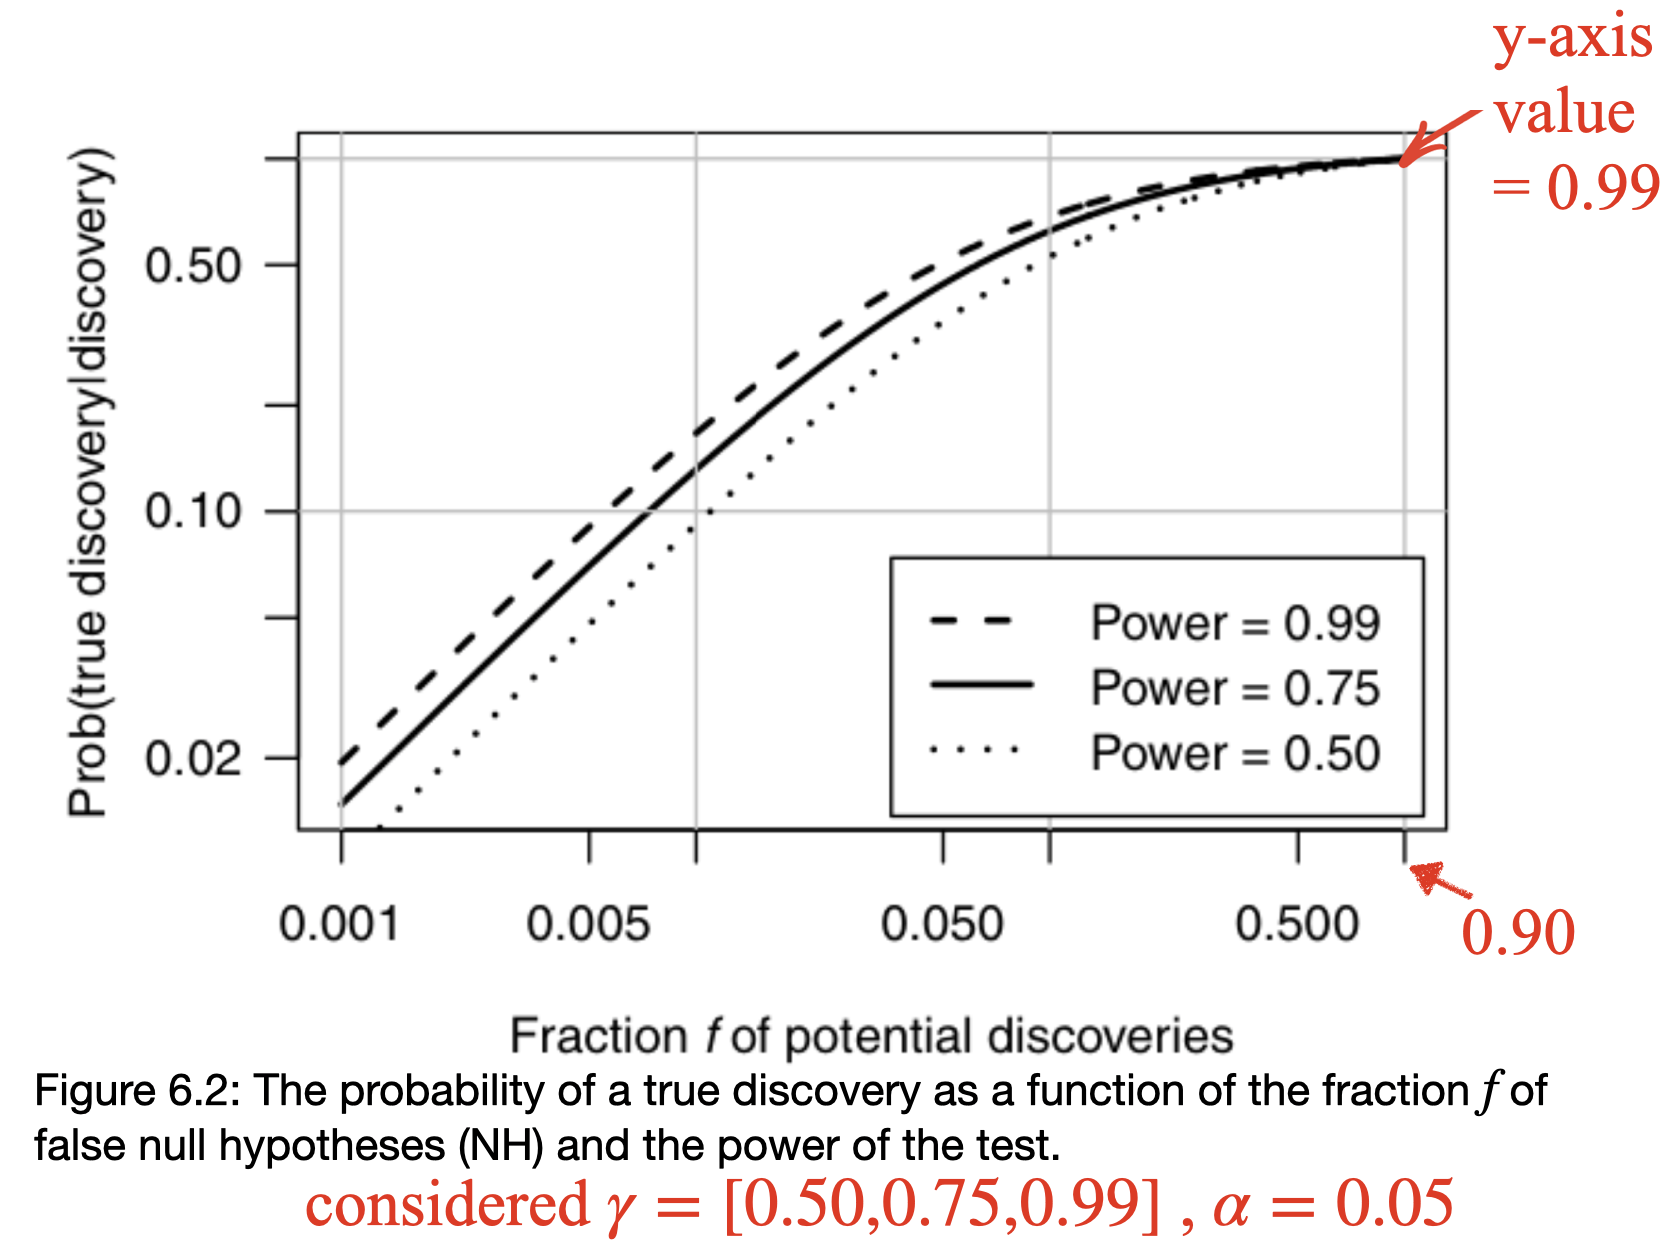
\includegraphics[width=0.65\textwidth]{fig6.png}
\end{figure}

\section*{Multiple Testing}
Multiple testing is a significant issue in interpreting tests. If 100 independent tests are conducted at $\alpha = 0.05$, and if $H_0$ is true in all cases, about $100 \times 0.05 = 5$ tests are expected to show significance purely by chance.

Traditional methods of surviving multiple testing are to control the \textit{family-wise error rate} rather than the \textit{per-test error rate}, but recent methodology is based on controlling the \textit{false discovery rate}. Except for testing for outliers, we leave discussion and application of multiple testing methods to other sources.

\end{document}